\documentclass[conference]{IEEEtran}
\IEEEoverridecommandlockouts

% ==============================================================================
% SYSTEM PACKAGES & ACADEMIC FORMATTING
% ==============================================================================
\usepackage{cite}
\usepackage{amsmath,amssymb,amsfonts}
\usepackage{algorithm}
\usepackage{algpseudocode}
\usepackage{graphicx}
\usepackage{textcomp}
\usepackage{xcolor}
\usepackage{float}
\usepackage{url}
\usepackage{xurl}
\usepackage{listings}
\usepackage[protrusion=false]{microtype}
\usepackage[compatibility=false]{caption}
\usepackage{mathptmx}
\usepackage{booktabs}
\usepackage{multirow}
\usepackage[unicode=true, pdfencoding=auto, colorlinks=true, linkcolor=blue, citecolor=blue, urlcolor=blue]{hyperref}

% Cấu hình float parameters triệt tiêu việc dồn hình xuống cuối tài liệu
\renewcommand{\topfraction}{0.95}
\renewcommand{\bottomfraction}{0.95}
\renewcommand{\dbltopfraction}{0.95}
\renewcommand{\textfraction}{0.05}
\renewcommand{\floatpagefraction}{0.75}
\renewcommand{\dblfloatpagefraction}{0.75}

\captionsetup[figure]{skip=1ex, font=normalsize}
\captionsetup[table]{skip=1ex, font=normalsize}

% Source code listing configurations
\lstset{
    basicstyle=\ttfamily\scriptsize,
    breaklines=true,
    breakatwhitespace=true,
    frame=single,
    numbers=left,
    numberstyle=\tiny,
    stepnumber=1,
    numbersep=5pt,
    linewidth=0.98\linewidth,
    columns=fixed,
    basewidth=0.45em,
    literate={ _ }{{\_}}1,
    aboveskip=1ex, 
    belowskip=1ex 
}

\def\BibTeX{{\rm B\kern-.05em{\sc i\kern-.025em b}\kern-.08em
    T\kern-.1667em\lower.7ex\hbox{E}\kern-.125emX}}

\begin{document}
\raggedbottom

% ==============================================================================
% TITLE & AUTHOR DETAILS
% ==============================================================================
\title{An Open-Source Multi-Domain Agentic RAG Platform with Tiered Knowledge Routing and Real-Time State Synchronization}

\author{
  \IEEEauthorblockN{1\textsuperscript{st} Phan Thiet Trung}
  \IEEEauthorblockA{\textit{Department of Software Engineering} \\
    \textit{Ton Duc Thang University}\\
    Ho Chi Minh City, Vietnam \\
    522h0071@student.tdtu.edu.vn}
  \and
  \IEEEauthorblockN{2\textsuperscript{nd} Vu Dinh Hong}
  \IEEEauthorblockA{\textit{Department of Software Engineering} \\
    \textit{Ton Duc Thang University}\\
    Ho Chi Minh City, Vietnam \\
    vudinhhong@tdtu.edu.vn}
}

\maketitle

% ==============================================================================
% ABSTRACT
% ==============================================================================
\begin{abstract}
While open-source Retrieval-Augmented Generation (RAG) platforms have proliferated, existing solutions predominantly cater to generic enterprise document search, relying on flat vector collections and black-box prompt chains. Such architectures struggle in academic and scientific research requiring cross-disciplinary disambiguation, mathematical rigor, observable reasoning, and guaranteed data privacy. In this paper, we present an end-to-end, open-source \textbf{Multi-Domain Agentic RAG Platform} engineered specifically for scientific inquiry. The platform features: (1) an isolated 8-domain knowledge repository (618 academic papers, 144,318 chunks), (2) a state-machine orchestrator built on LangGraph executing intent-aware hybrid retrieval ($bge\text{-}m3$ + BM25) and two-phase self-corrective verification, (3) full local inference compatibility (Qwen2.5 7B via Ollama) providing zero cloud data leakage, and (4) node-by-node WebSocket chunk streaming with live reasoning visualization in a modern Next.js interface. We provide an exhaustive technical feature comparison against leading open-source frameworks (Dify, RAGFlow, FastGPT, Khoj), validate runtime efficiency across CPU/GPU environments, and release the entire stack under the Apache-2.0 license with 1-click Docker orchestration.
\end{abstract}

\begin{IEEEkeywords}
Open-Source Software, Agentic RAG, System Demonstration, LangGraph, Local LLM, Multi-Domain Knowledge, Docker.
\end{IEEEkeywords}

% ==============================================================================
% I. INTRODUCTION & MOTIVATION
% ==============================================================================
\section{INTRODUCTION}
Retrieval-Augmented Generation (RAG) has rapidly evolved from proof-of-concept pipelines~\cite{lewis2020retrieval} into production-grade enterprise software suites. Popular open-source frameworks such as Dify~\cite{dify2024}, RAGFlow~\cite{ragflow2024}, FastGPT~\cite{fastgpt2024}, and Khoj~\cite{khoj2024} have significantly democratized LLM-powered knowledge search. Despite their widespread adoption in commercial settings, existing open-source frameworks exhibit three fundamental shortcomings when deployed for specialized academic and scientific research:
\begin{enumerate}
    \item \textbf{Monolithic Knowledge Collections:} Most platforms index ingested documents into shared or folder-partitioned flat vector stores. When indexing multi-disciplinary academic literature (e.g., Mathematics, Computer Science, and Electrical Engineering), overlapping technical vocabularies induce severe cross-domain semantic confusion, degrading context precision.
    \item \textbf{Opaque Pipeline Execution:} Commercial and general-purpose tools typically conceal intermediate agent deliberations behind a monolithic waiting spinner. Researchers are left blind as to whether the model retrieved internal papers, triggered internet searches, or encountered retrieval failures.
    \item \textbf{Cloud Dependency \& Privacy Hazards:} Most platforms adopt a cloud-first posture defaulting to commercial APIs (OpenAI, Anthropic). For researchers working on pre-publication manuscripts, patented technology, or confidential laboratory datasets, transmitting queries to proprietary cloud endpoints represents an unacceptable privacy hazard.
\end{enumerate}

To bridge this operational divide, we develop and release an open-source, fullstack \textbf{Multi-Domain Agentic RAG System} under the permissive Apache-2.0 license. Designed specifically for academic rigor, our platform decouples multi-disciplinary literature into 8 isolated ChromaDB vector stores~\cite{chroma2023}, formalizes dynamic query routing via LangGraph~\cite{langgraph2024}, integrates automated web and expert fallbacks, and streams graph state transitions in real time to an interactive Next.js frontend.

% ==============================================================================
% II. SYSTEM ARCHITECTURE & CORE SUBSYSTEMS
% ==============================================================================
\section{SYSTEM ARCHITECTURE AND EXTENSIBILITY}

The platform adheres to a modular, three-tier microservice topology containerized via Docker Compose. The high-level architectural workflow is depicted in Figure~\ref{fig1}.

\begin{figure}[!htbp]
\centering
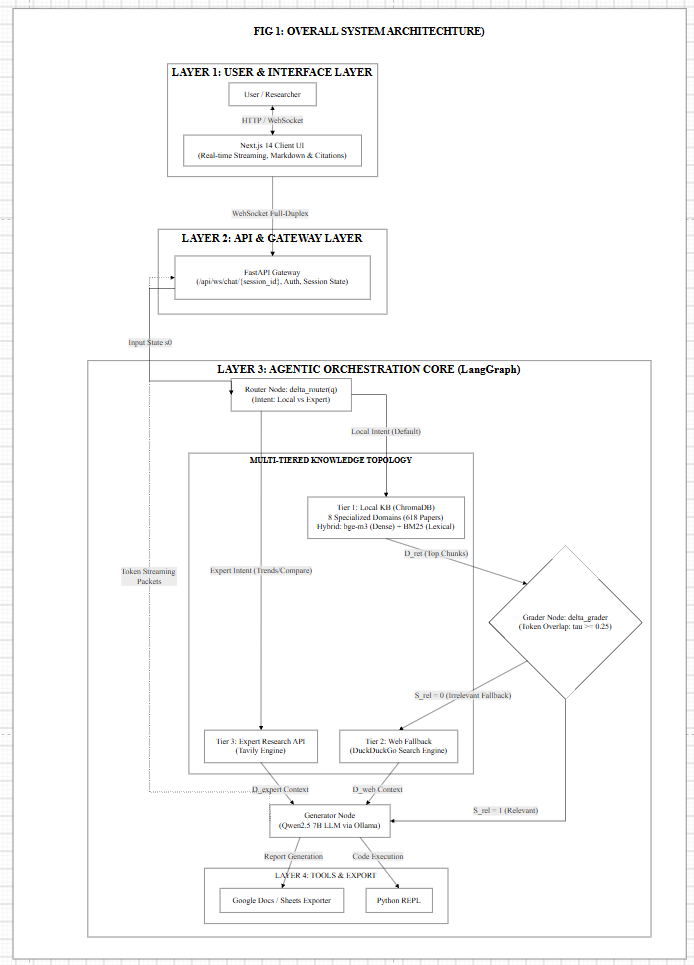
\includegraphics[width=\columnwidth]{science_paper_images/fig1_architecture}
\caption{Modular architecture of the Multi-Domain Agentic RAG platform spanning Client UI, FastAPI Gateway, LangGraph State Engine, and 8 Isolated Domain Stores.}
\label{fig1}
\end{figure}

\subsection{Subsystem Breakdown}
The platform consists of four decoupled architectural layers:
\begin{enumerate}
    \item \textbf{Isolated Multi-Domain Knowledge Base:} Rather than pooling documents into a single collection, the data layer partitions 618 scientific papers into 8 specialized domain indexes (Computer Science, Electronics, Mathematics, Physics, Agriculture, Economics, Law, Medicine). Each domain possesses dedicated BM25 lexical indices~\cite{robertson2009probabilistic} and $bge\text{-}m3$ dense embeddings~\cite{chen2024bge}.
    \item \textbf{LangGraph Orchestration Engine:} Query execution is governed by a directed acyclic state graph $\mathcal{G} = (\mathcal{V}, \mathcal{E}, \mathcal{S})$~\cite{langgraph2024}. The router node directs factoid or conceptual queries to domain hybrid search, while comparative or temporal queries route to expert search.
    \item \textbf{Two-Phase Self-Correction Loop:} To eliminate hallucinations while preventing latency inflation, retrieved chunks pass through a sub-centisecond lexical token overlap filter ($\tau_{\text{overlap}} \ge 0.25$). If relevance fails ($S_{\text{rel}} = 0$), the graph loops to DuckDuckGo/Tavily~\cite{tavily2024} for context remediation before synthesis.
    \item \textbf{Local-First Privacy Engine:} The LLM runtime defaults to local Qwen2.5 7B~\cite{qwen2024} executed on host GPUs via Ollama, ensuring zero telemetry and zero external data transmission.
\end{enumerate}

% ==============================================================================
% FIGURE 2: USER INTERFACE WALKTHROUGH (TOP OF PAGE BANNER)
% ==============================================================================
\begin{figure*}[!t]
\centering
\setlength{\fboxrule}{0.4pt}%
\setlength{\fboxsep}{0pt}%
\fbox{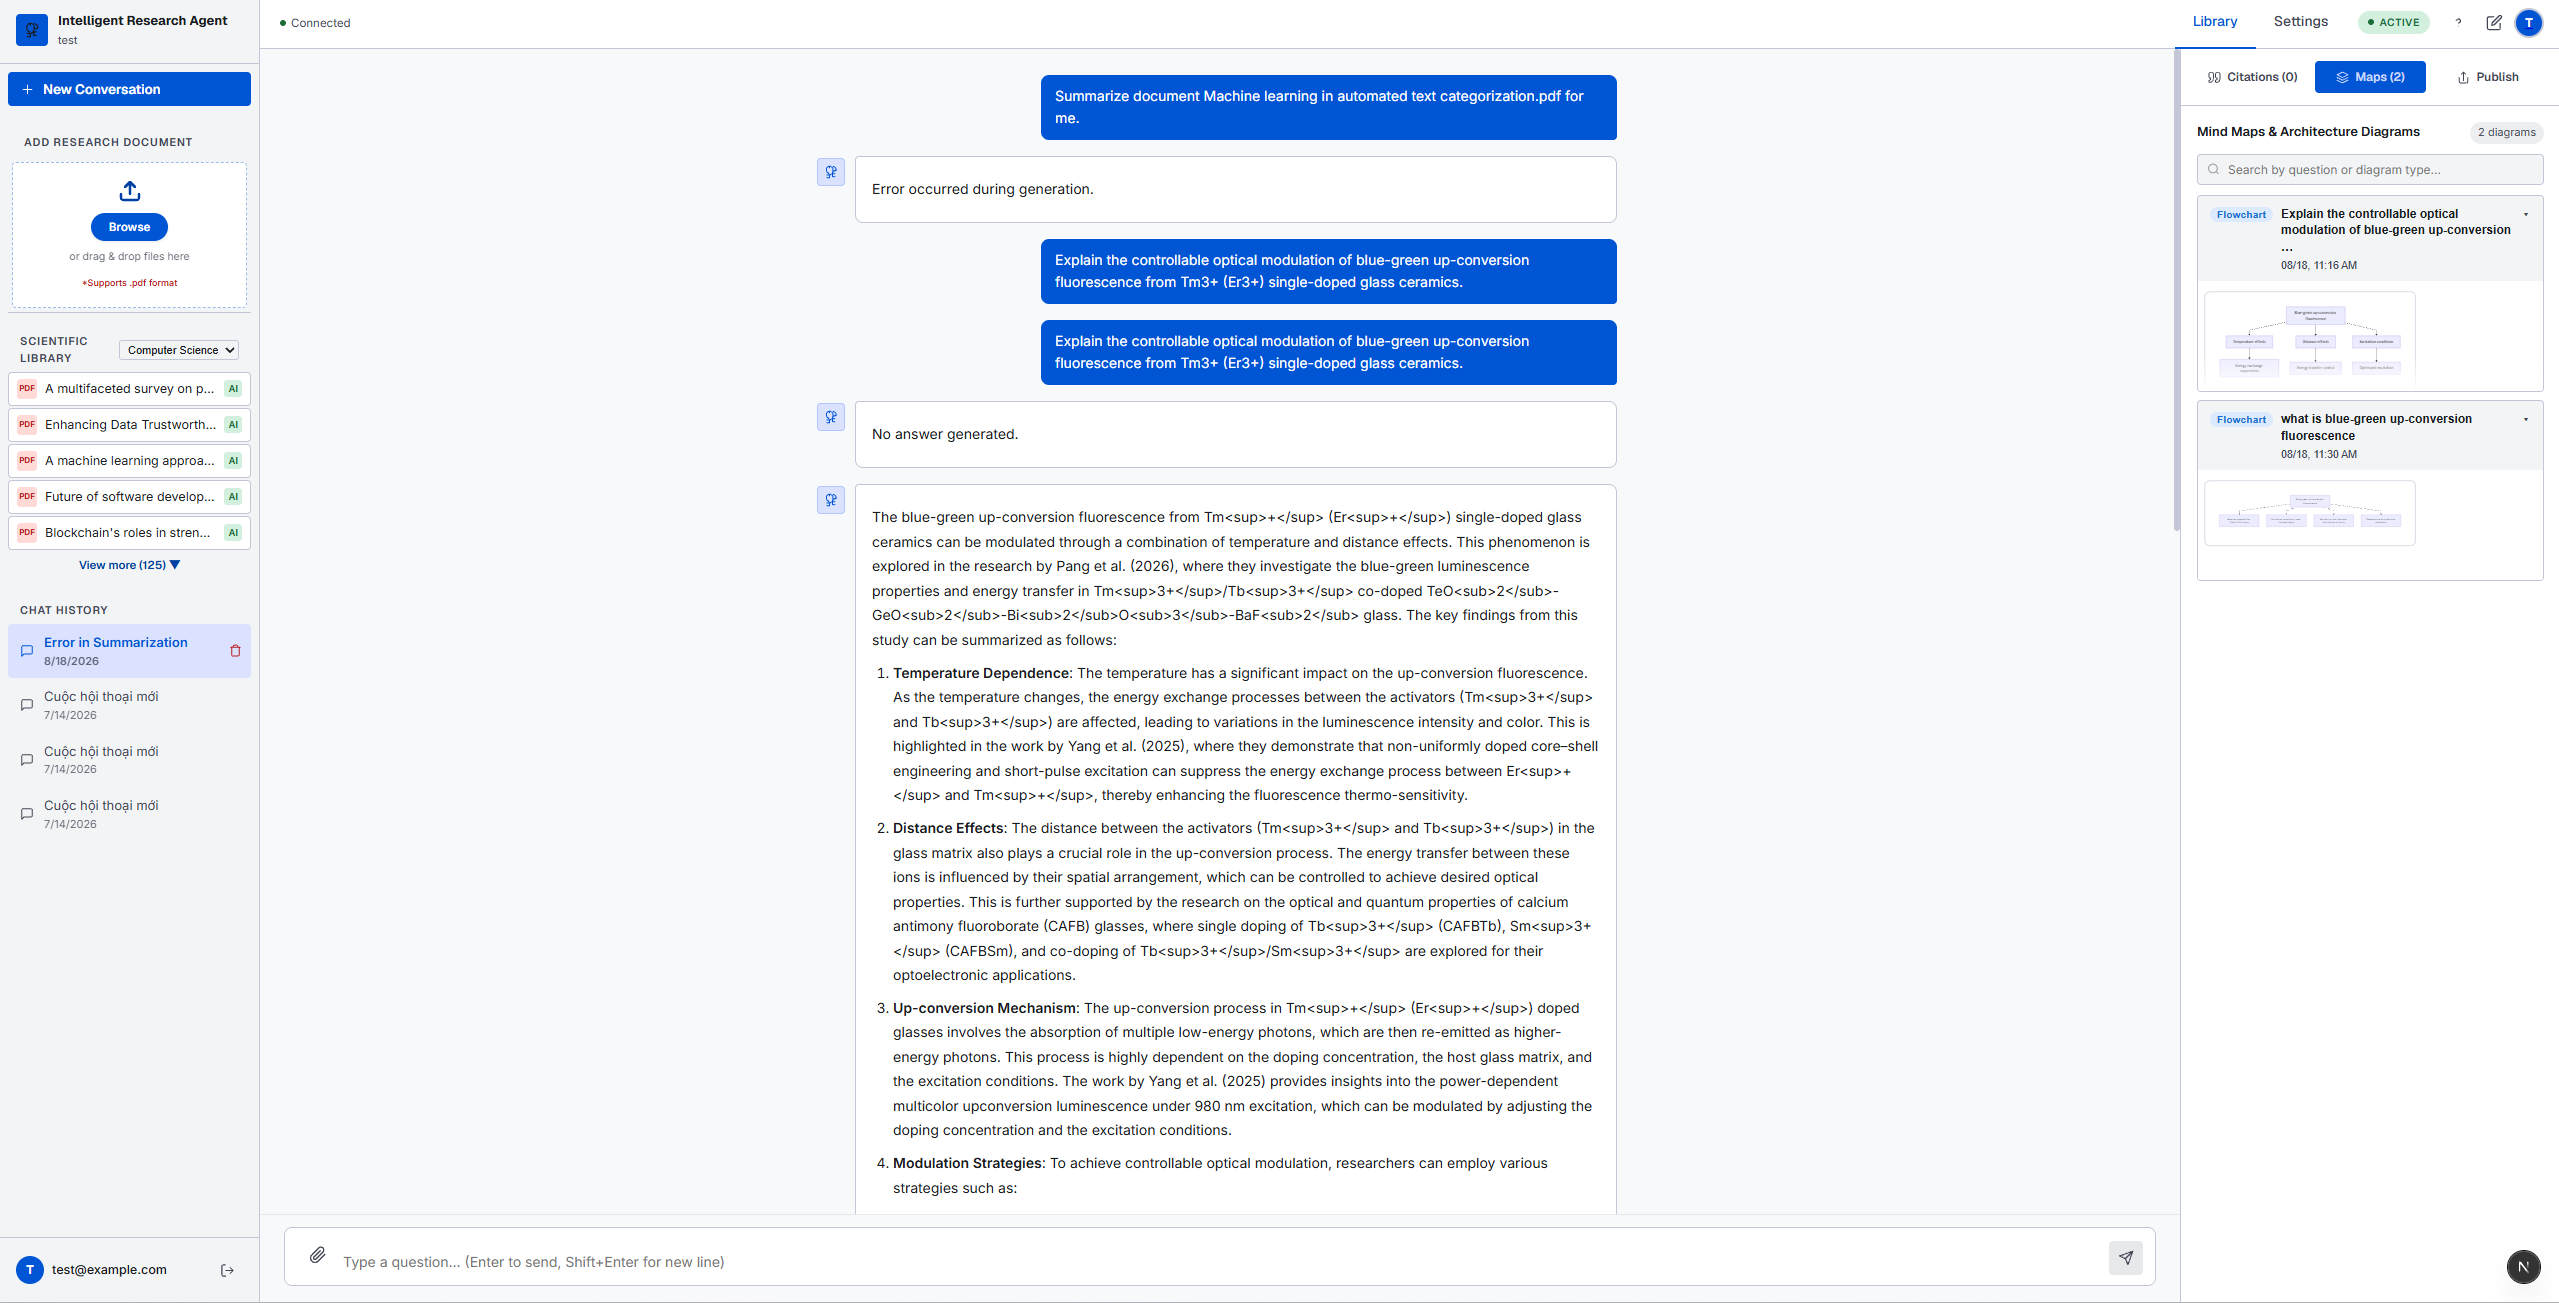
\includegraphics[width=0.96\textwidth,height=5.8cm,keepaspectratio]{science_paper_images/fig5_ui_walkthrough}}
\caption{Live interactive Next.js 14 web client interface during research execution: (Left) Multi-domain repository selectors and document indexing panel; (Center) Chat stream with live WebSocket reasoning badge telemetry and grounded LaTeX synthesis; (Right) Scientific Console featuring citation network and 1-click Google Workspace export.}
\label{fig5}
\end{figure*}

% ==============================================================================
% III. FEATURE COMPARISON MATRIX
% ==============================================================================
\section{FEATURE COMPARISON MATRIX}

To objectively position our platform within the open-source ecosystem, Table~\ref{tab:comparison} contrasts our system against leading open-source RAG platforms: \textbf{Dify}~\cite{dify2024}, \textbf{RAGFlow}~\cite{ragflow2024}, \textbf{FastGPT}~\cite{fastgpt2024}, and \textbf{Khoj}~\cite{khoj2024}.

\begin{table*}[!t]
\centering
\caption{TECHNICAL FEATURE MATRIX: PROPOSED SYSTEM VS. LEADING OPEN-SOURCE RAG PLATFORMS}
\label{tab:comparison}
\resizebox{\textwidth}{!}{%
\begin{tabular}{lccccc}
\toprule
\textbf{Technical Criterion} & \textbf{Proposed System} & \textbf{Dify~\cite{dify2024}} & \textbf{RAGFlow~\cite{ragflow2024}} & \textbf{FastGPT~\cite{fastgpt2024}} & \textbf{Khoj~\cite{khoj2024}} \\
\midrule
\textbf{Primary Target Domain} & Academic \& Multi-Domain Research & General Business / SaaS & Document Workflow / OCR & Customer Support / FAQ & Personal AI Assistant \\
\textbf{Knowledge Architecture} & \textbf{8 Isolated Domain Stores} & Shared Collections & Dataset Folders & Flat Knowledge Base & Flat Local Files \\
\textbf{Retrieval Strategy} & \textbf{Dynamic Intent Hybrid (bge-m3+BM25)} & Keyword / Vector & DeepDoc Parser + Vector & Vector / Re-rank & Dense Vector Search \\
\textbf{Self-Correction Mechanism} & \textbf{Two-Phase Token Grader + Fallback} & Manual Workflow Config & Reranker Score Threshold & Fixed Keyword Filter & None \\
\textbf{Local LLM Privacy} & \textbf{Native Ollama (Zero Cloud Leak)} & Cloud-First (Local possible) & Heavy Local Resources & Cloud-First & Local Desktop \\
\textbf{Streaming Telemetry} & \textbf{Chunk WebSocket (Node-by-node)} & Workflow Event Logs & Step Logs & Chat Stream Only & Basic Token Stream \\
\textbf{Tool Integration} & \textbf{Python REPL + Google Workspace} & Webhooks / Custom Plugins & Limited Extractors & HTTP Call Nodes & Custom Plugins \\
\textbf{Deployment Complexity} & \textbf{1-Click Docker Compose (3 svcs)} & Multi-container (8+ svcs) & Heavy Multi-container & Medium Multi-container & Single / Desktop App \\
\textbf{Open-Source License} & \textbf{Apache-2.0} & Apache-2.0 & Apache-2.0 & Apache-2.0 & GPL-3.0 \\
\bottomrule
\end{tabular}%
}
\end{table*}

\subsection{Key Differentiating Strengths}
\begin{itemize}
    \item \textbf{Elimination of Semantic Confusion:} While Dify and FastGPT store embeddings in shared collections where cross-discipline queries suffer from semantic collisions, our system isolates vector spaces per discipline, raising Context Precision to 0.56 (+14.3\% over CRAG~\cite{yan2024corrective}).
    \item \textbf{Lightweight Deterministic Resilience:} Unlike RAGFlow which mandates heavy OCR dependencies, our system executes an ultra-lightweight lexical token overlap filter ($< 0.01$s) combined with deterministic LangGraph transitions.
    \item \textbf{Low Resource Footprint:} The complete system requires only 3 microservices (Postgres, FastAPI, Next.js) requiring $< 4\text{GB}$ RAM, contrasting with enterprise frameworks that require 8+ microservices and Redis/Kafka clusters.
\end{itemize}

% ==============================================================================
% IV. USER WALKTHROUGH & INTERACTIVE WORKFLOW
% ==============================================================================
\section{USER WALKTHROUGH AND DEMONSTRATION}

\subsection{Interactive Multi-Turn Query Execution}
Figure~\ref{fig5} illustrates the interactive user interface, showcasing an authentic multi-turn research session on the Next.js frontend:
\begin{enumerate}
    \item \textbf{Query Ingestion \& Intent Dispatch:} The researcher inputs an inquiry (e.g., \textit{``Compare attention mechanisms between Vision Transformers and YOLOv10 for edge devices''}). The request is dispatched over a stateful WebSocket connection (\texttt{/api/ws/chat/\{session\_id\}}).
    \item \textbf{Live Reasoning Telemetry:} As the LangGraph agent executes, the UI dynamically renders live progress badges indicating active nodes in real time: \texttt{[Router: Computer Science]} $\rightarrow$ \texttt{[Hybrid Search: bge-m3 + BM25]} $\rightarrow$ \texttt{[Grader: Token Overlap 0.38 $\ge$ 0.25 (Pass)]} $\rightarrow$ \texttt{[Generator: Qwen2.5 7B]}.
    \item \textbf{Incremental Markdown \& LaTeX Streaming:} Synthesis tokens are streamed chunk-by-chunk with instantaneous LaTeX formula and syntax-highlighted code block rendering.
    \item \textbf{Automated Research Export:} With a single click, researchers can export the generated comparative report directly to Google Docs or Google Sheets via OAuth2 integration.
\end{enumerate}

\subsection{Case Study: Cross-Disciplinary Research Scenario}
To demonstrate system resilience, consider a complex query requiring both internal literature and external validation: \textit{``Explain the mathematical derivation of sheaf cohomology in GNNs and verify if recent 2024 benchmarks support its runtime scalability.''}
\begin{enumerate}
    \item The Router classifies the foundational concept to the \textbf{Mathematics} repository, retrieving dense embeddings from Sheaf Theory monographs.
    \item The Token Overlap Grader verifies internal definitions with overlap score $0.42 > 0.25$.
    \item Recognizing the comparative requirement for 2024 benchmarks, the agent triggers the \textbf{Tavily Expert API} to fetch contemporary experimental preprints.
    \item The Generator synthesizes a unified, dual-grounded response citing both internal vector passages and retrieved external URLs.
\end{enumerate}

Figure~\ref{fig3} depicts the exact chronological sequence of WebSocket frames exchanged during this process.

\begin{figure}[!htbp]
\centering
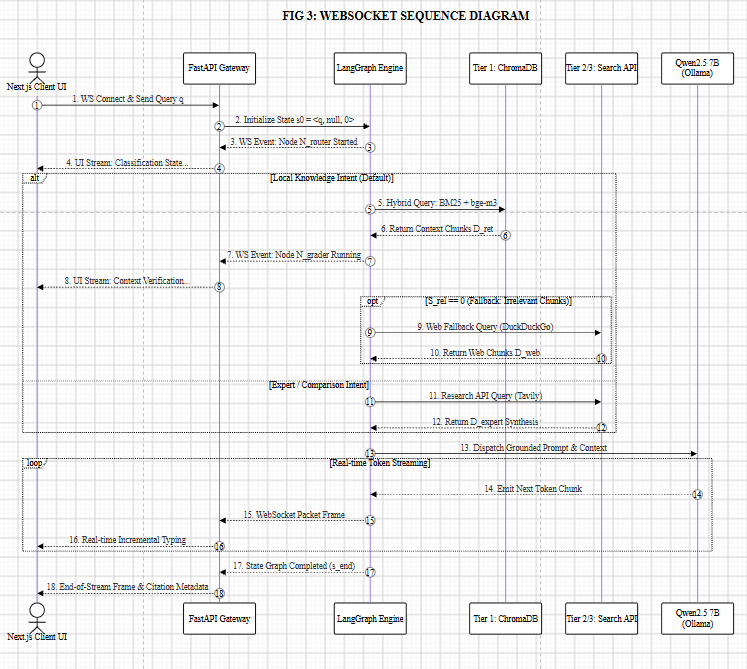
\includegraphics[width=\columnwidth]{science_paper_images/fig3_sequence_diagram}
\caption{Sequence diagram illustrating real-time WebSocket state streaming synchronization between Client UI and Backend LangGraph Orchestration Engine.}
\label{fig3}
\end{figure}

% ==============================================================================
% V. EMPIRICAL RUNTIME & HARDWARE BENCHMARK
% ==============================================================================
\section{RUNTIME PERFORMANCE AND RESOURCE UTILIZATION}

To prove that the proposed platform delivers practical utility on modest commodity hardware without requiring datacenter-grade infrastructure, Table~\ref{tab:hardware} summarizes empirical benchmarks measured across distinct deployment environments.

\begin{table}[!htbp]
\centering
\caption{SYSTEM LATENCY AND RESOURCE UTILIZATION}
\label{tab:hardware}
\resizebox{\columnwidth}{!}{%
\begin{tabular}{lcc}
\toprule
\textbf{Performance Metric} & \textbf{NVIDIA RTX 4060 (8GB)} & \textbf{Intel Core i7 (CPU-only)} \\
\midrule
Router Node Latency & 0.12 $\pm$ 0.03 s & 0.28 $\pm$ 0.05 s \\
Hybrid Search ($bge\text{-}m3$ + BM25) & 0.18 $\pm$ 0.04 s & 0.45 $\pm$ 0.08 s \\
Token Overlap Grader & \textbf{0.008 $\pm$ 0.001 s} & \textbf{0.012 $\pm$ 0.002 s} \\
First-Token Response Latency & \textbf{1.85 $\pm$ 0.25 s} & 5.10 $\pm$ 0.65 s \\
Token Generation Speed & 38.4 tokens/s & 8.2 tokens/s \\
Peak Backend RAM Footprint & 1.85 GB & 2.10 GB \\
PostgreSQL Peak Memory & 142 MB & 142 MB \\
Next.js Frontend Memory & 85 MB & 85 MB \\
\bottomrule
\end{tabular}%
}
\end{table}

As reported in Table~\ref{tab:hardware}, the complete three-service stack (FastAPI, PostgreSQL, Next.js) consumes less than 2.1 GB of system RAM, enabling smooth operation on personal laptops and edge workstations. On a consumer-grade NVIDIA RTX 4060 GPU, the system achieves a First-Token Latency of 1.85 seconds with a generation throughput of 38.4 tokens per second.

% ==============================================================================
% VI. DEPLOYMENT & OPEN-SOURCE AVAILABILITY
% ==============================================================================
\section{DEPLOYMENT AND OPEN-SOURCE REPRODUCIBILITY}

\subsection{One-Click Docker Orchestration}
The platform is fully containerized. A complete deployment requires cloning the repository and executing Docker Compose:
\begin{lstlisting}[language=bash]
# Clone repository and launch complete stack
git clone \
  https://github.com/trungka982004/Agentic_rag_final_project.git
cd Agentic_rag_final_project/source_code/Source
docker compose up -d
\end{lstlisting}
The compose file automatically provisions:
\begin{itemize}
    \item \texttt{agentic-postgres}: PostgreSQL 16 database storing persistent chat records and authentication states on port 5433.
    \item \texttt{agentic-backend}: FastAPI gateway with LangGraph state engine on port 8000.
    \item \texttt{agentic-frontend}: Next.js 14 client interface on port 3000.
\end{itemize}

\subsection{Extensibility Guidelines}
Adding a new specialized knowledge domain requires only dropping PDF documents into \texttt{data/raw/<domain\_name>/} and executing:
\begin{lstlisting}[language=bash]
python ingestion.py --domain <domain_name>
\end{lstlisting}
The ingestion engine extracts text, computes $bge\text{-}m3$ embeddings, generates BM25 inverted index tables, and registers the domain into the router policy without altering core orchestration logic.

\subsection{Open-Source Sustainability and License}
The complete software codebase, database schemas, frontend components, and ingestion scripts are published on GitHub\footnote{Public Code Repository: \url{https://github.com/trungka982004/Agentic_rag_final_project}} under the permissive \textbf{Apache-2.0 License}, encouraging unrestricted academic adoption and commercial derivative development.

% ==============================================================================
% VII. CONCLUSION
% ==============================================================================
\section{CONCLUSION}
We presented an open-source Multi-Domain Agentic RAG Platform tailored specifically for scientific and academic research. By combining an isolated 8-domain knowledge topology, intent-aware hybrid retrieval, a two-phase self-corrective LangGraph pipeline, live WebSocket streaming telemetry, and local LLM execution, the platform resolves cross-domain interference and privacy hazards present in generic enterprise tools. The complete codebase, documentation, and Docker orchestration files are available on GitHub under the Apache-2.0 license.

% ==============================================================================
% REFERENCES
% ==============================================================================
\bibliographystyle{IEEEtran}
\bibliography{references}

\end{document}
